%%%%%%%%%%%%%%%%%%%%%%%%%%%%%%%%%%%%%%%%%%%%%%%%%%%%%%%%%%%%%%%%%%%%%%%%%%%%%%%%
%2345678901234567890123456789012345678901234567890123456789012345678901234567890
%        1         2         3         4         5         6         7         8

\documentclass[letterpaper, 10 pt, conference]{ieeeconf}  % Comment this line out if you need a4paper

%\documentclass[a4paper, 10pt, conference]{ieeeconf}      % Use this line for a4 paper

\IEEEoverridecommandlockouts                              % This command is only needed if
                                                          % you want to use the \thanks command

\overrideIEEEmargins                                      % Needed to meet printer requirements.

%In case you encounter the following error:
%Error 1010 The PDF file may be corrupt (unable to open PDF file) OR
%Error 1000 An error occurred while parsing a contents stream. Unable to analyze the PDF file.
%This is a known problem with pdfLaTeX conversion filter. The file cannot be opened with acrobat reader
%Please use one of the alternatives below to circumvent this error by uncommenting one or the other
%\pdfobjcompresslevel=0
%\pdfminorversion=4

% See the \addtolength command later in the file to balance the column lengths
% on the last page of the document

% The following packages can be found on http:\\www.ctan.org
%\usepackage{graphics} % for pdf, bitmapped graphics files
%\usepackage{epsfig} % for postscript graphics files
%\usepackage{mathptmx} % assumes new font selection scheme installed
%\usepackage{times} % assumes new font selection scheme installed
%\usepackage{amsmath} % assumes amsmath package installed
%\usepackage{amssymb}  % assumes amsmath package installed

\usepackage[normalem]{ulem} % for strikethrough while editting
\usepackage{graphicx}
\usepackage{cuted}
\usepackage{capt-of}
\setlength{\stripsep}{4pt plus 1pt minus 1pt}
\usepackage{flafter} % Makes figures appear after their references
\usepackage{dblfloatfix} % Force teaser image above abstract

\title{\LARGE \bf
Improving VLA Performance by Rephrasing Task Instructions
}


\author{Mikey Watts$^{1}$ and Mikey Watts$^{2}$% <-this % stops a space
\thanks{*This work was not supported by any organization}% <-this % stops a space
\thanks{$^{1}$Mikey Watts is an independent researcher in Los Angeles
        {\tt\small mikeywatts@berkeley.edu}}%
}


\graphicspath{{./}{../results/charts/}}

\begin{document}



\maketitle

\begin{strip}
    \vspace{-1.2em}
    \centering
    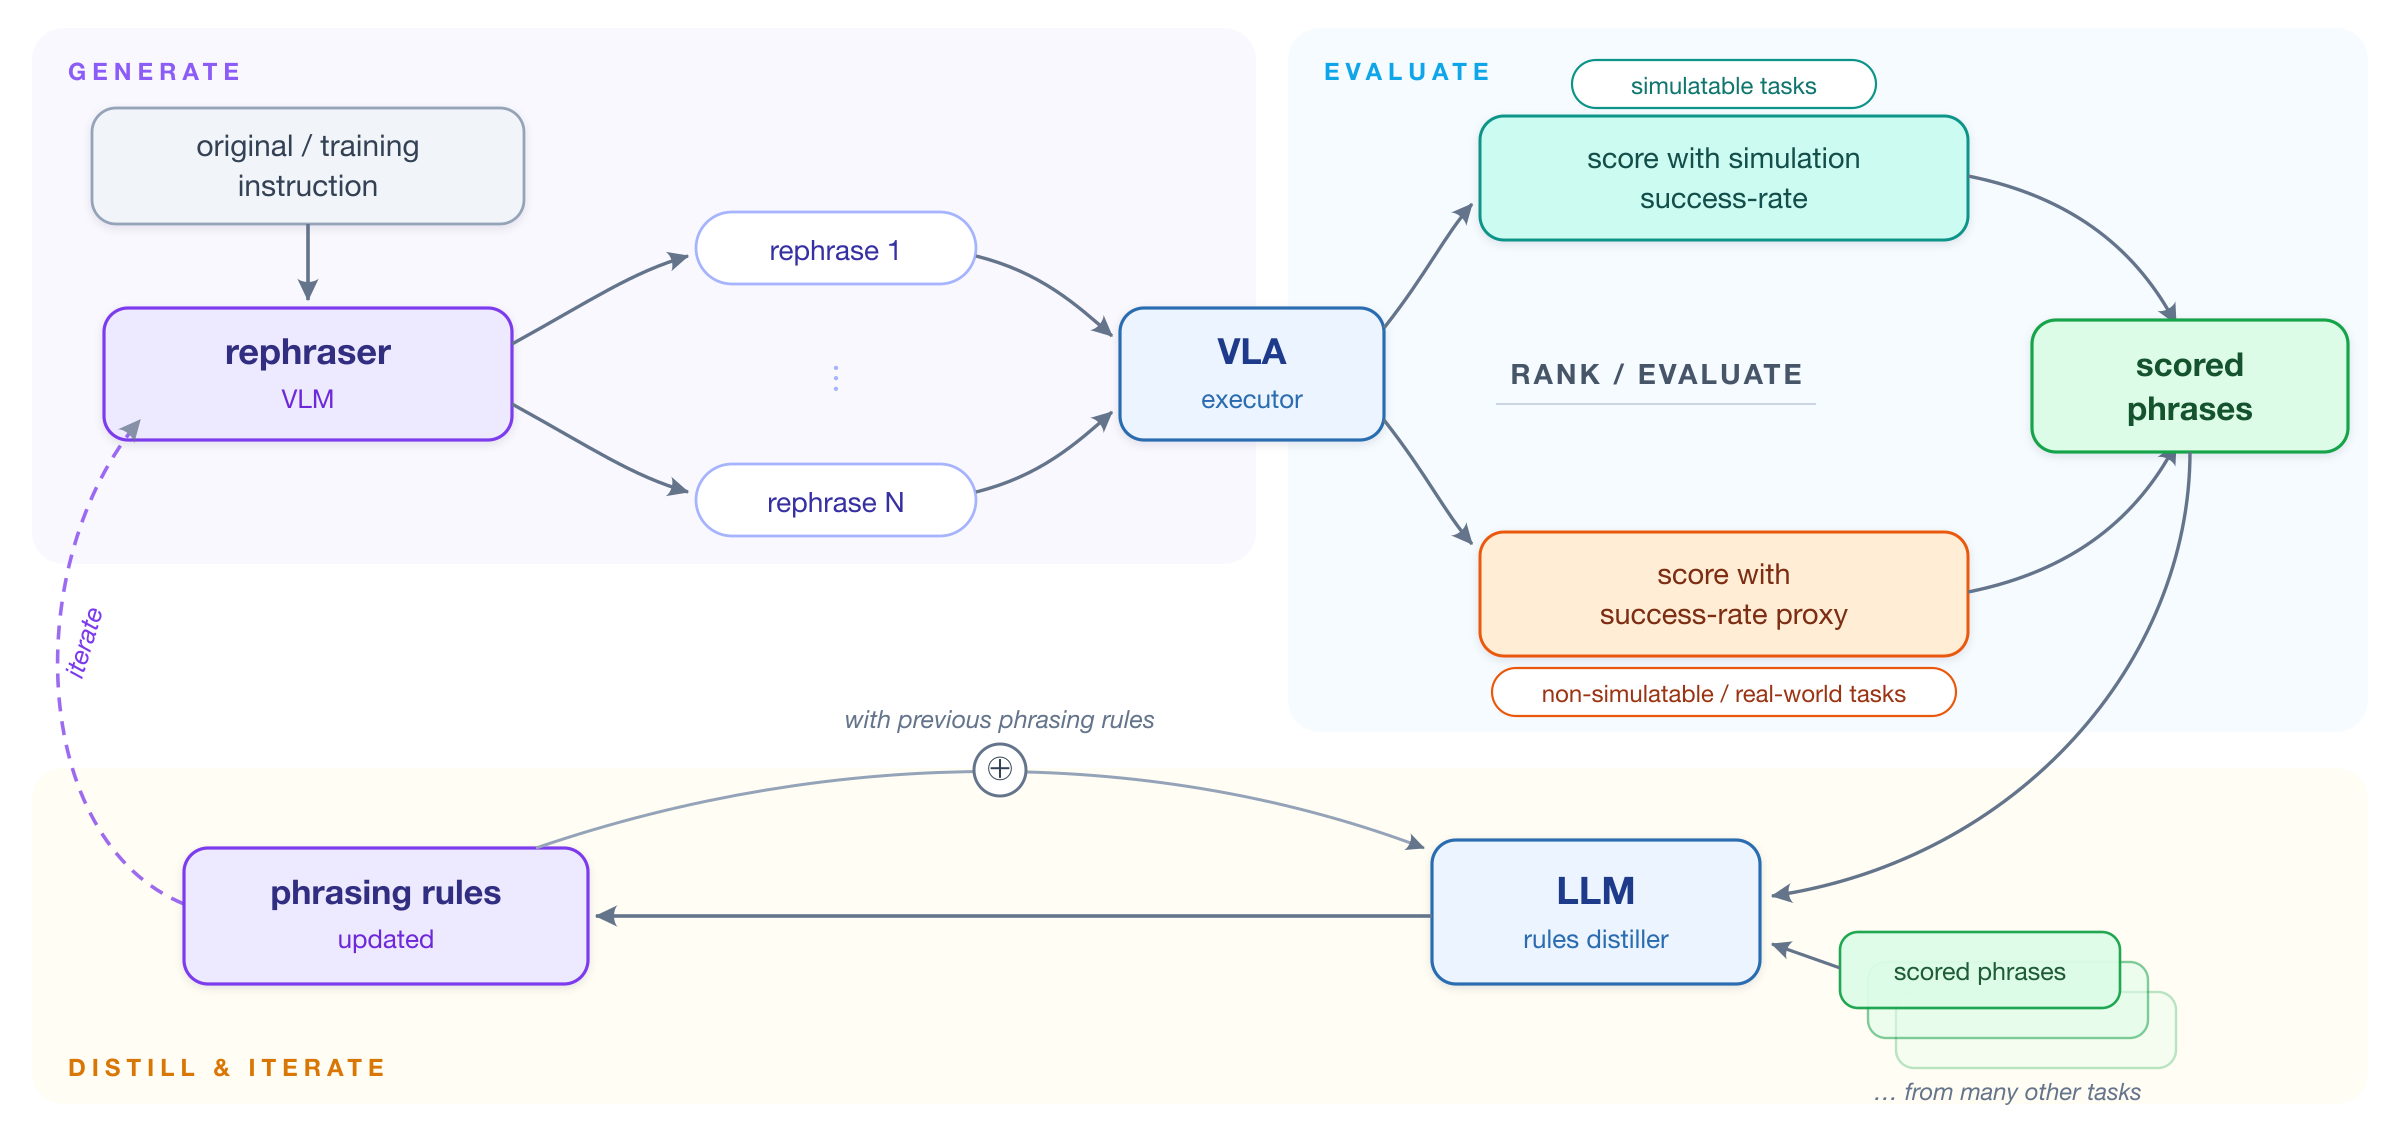
\includegraphics[width=\textwidth]{training_flow_compact.png}
    \captionof{figure}{Phrase-search and rule-distillation training loop.
    A VLM generates candidate rephrasings, which are evaluated using either
    simulation success rate or a learned success-rate proxy. An LLM distills
    the resulting scored phrases into updated phrasing rules for subsequent
    iterations.}
    \label{fig:training_flow_compact}
    \vspace{-0.5em}
\end{strip}

\begin{figure}[!t]
    \centering
    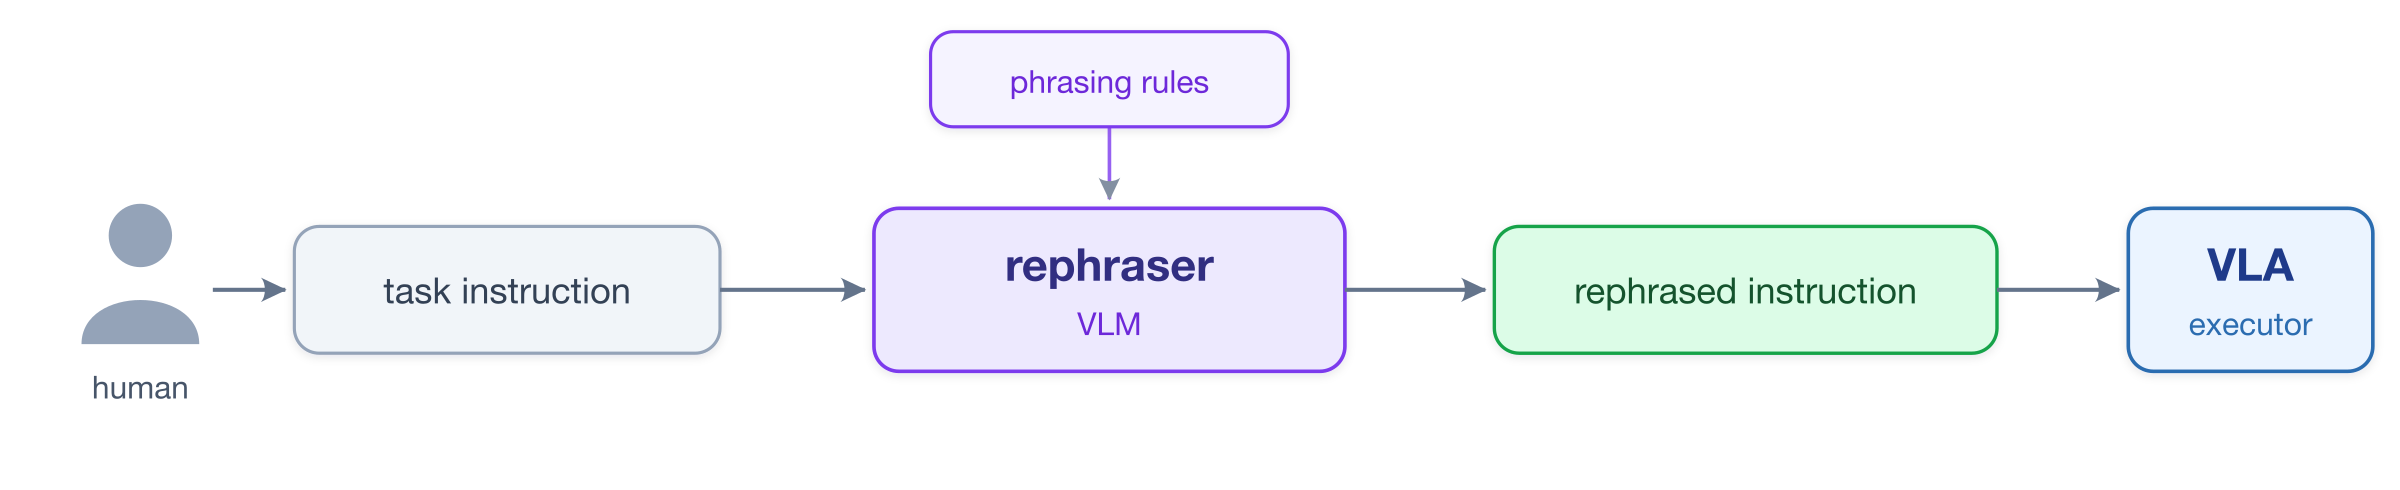
\includegraphics[width=\columnwidth]{inference_flow.png}
    \caption{At deployment time, a rephraser --- a VLM conditioned on
phrasing rules, or finetuned via SFT or GRPO --- rewrites each task
instruction before it reaches the VLA.}
    \label{fig:deployment}
\end{figure}


\thispagestyle{empty}
\pagestyle{empty}


%%%%%%%%%%%%%%%%%%%%%%%%%%%%%%%%%%%%%%%%%%%%%%%%%%%%%%%%%%%%%%%%%%%%%%%%%%%%%%%%
\begin{abstract}

Much progress has been made towards building general purpose robots. These robots are capable of being instructed by humans via natural language to perform a wide variety of tasks. However, many of the state of the art, open robots, implemented as Vision-Language-Action models (VLAs), are still very sensitive to instruction phrasing: variation in task phrasing can increase task success rates by up to 60\%. We highlight this gap across multiple models and datasets. We then compare three different methods of learning a given VLA's preferred language. We package these learnings into a "rephraser" that sits between the human and the robot, translating each instruction into the VLA's preferred phrasing. Our best method improves VLA performance on adversarially phrased instructions by 25\% and improves performance on naturally phrased instructions by 30\%.

\end{abstract}


%%%%%%%%%%%%%%%%%%%%%%%%%%%%%%%%%%%%%%%%%%%%%%%%%%%%%%%%%%%%%%%%%%%%%%%%%%%%%%%%
\section{Introduction}

We have come a long way toward developing general-purpose robots -- implemented as Vision-Language-Action models (VLAs) -- that can be instructed via natural language to perform a wide variety of tasks. These robots are built on top of Large Language Models (LLMs) which themselves demonstrate a super-human command of language. However, there's something lacking in the way that LLM's language skills transfer to VLAs: \sout{modern VLAs} $\pi_0$ is extremely sensitive to the specific phrasing of its given natural language instruction. As shown in Fig.~\ref{fig:pi0_conditions}, changes to task phrasing can affect \sout{VLA} $\pi_0$ performance by up to about 60\%; see Fig.~\ref{fig:spread_coke_can_on_keyboard}, ~\ref{fig:spread_cube_on_plate}, and ~\ref{fig:spread_eggplant_on_keyboard} for examples. Despite the fact that a VLA may have the required motor skills to perform a task, it is often not straightforward to find the optimal language instruction to trigger the skill.

\begin{figure}[!t]
    \centering
    
\includegraphics[width=\columnwidth]{pi0_conditions.png}
    \caption{Task phrasing significantly affects $\pi_0$ performance on the SIMPLER dataset. On out of vocabulary tasks, oracle phrasings improve task performance by more than 2x when compared to 16 natural phrasings. All evaluation are on 12 layouts of 12 tasks.}
    \label{fig:pi0_conditions}
\end{figure}

\begin{figure}[!t]
    \centering
    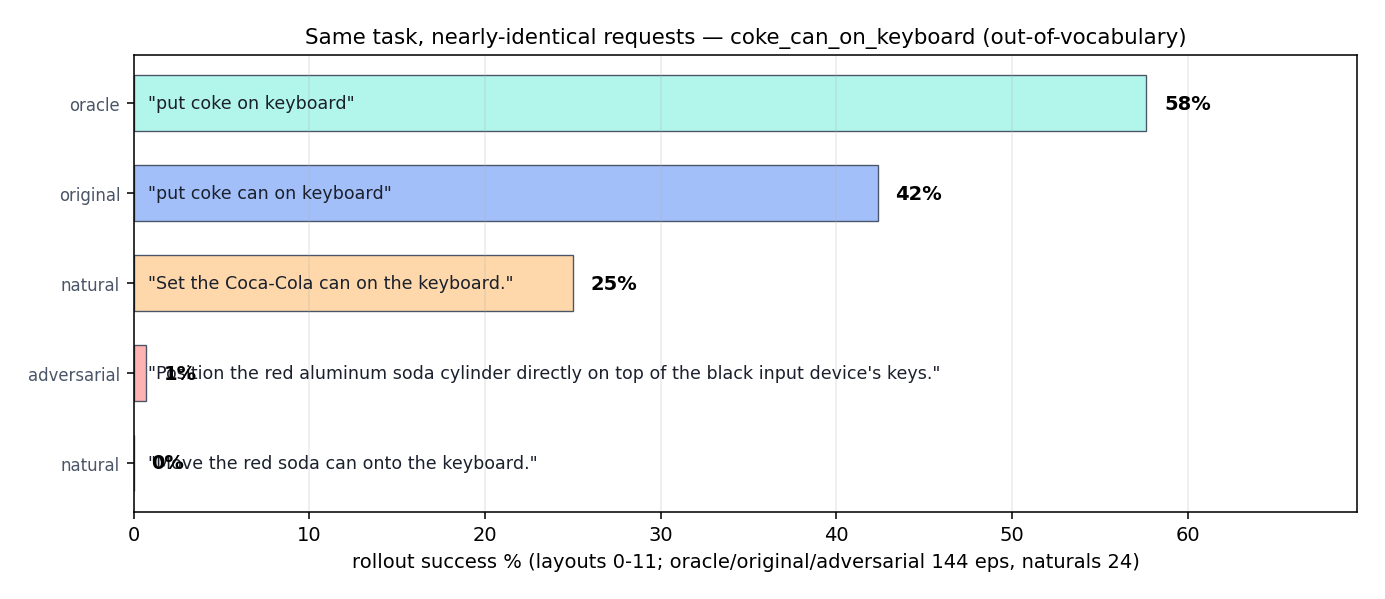
\includegraphics[width=\columnwidth]{spread_coke_can_on_keyboard.png}
    \caption{}
    \label{fig:spread_coke_can_on_keyboard}
\end{figure}

\begin{figure}[!t]
    \centering
    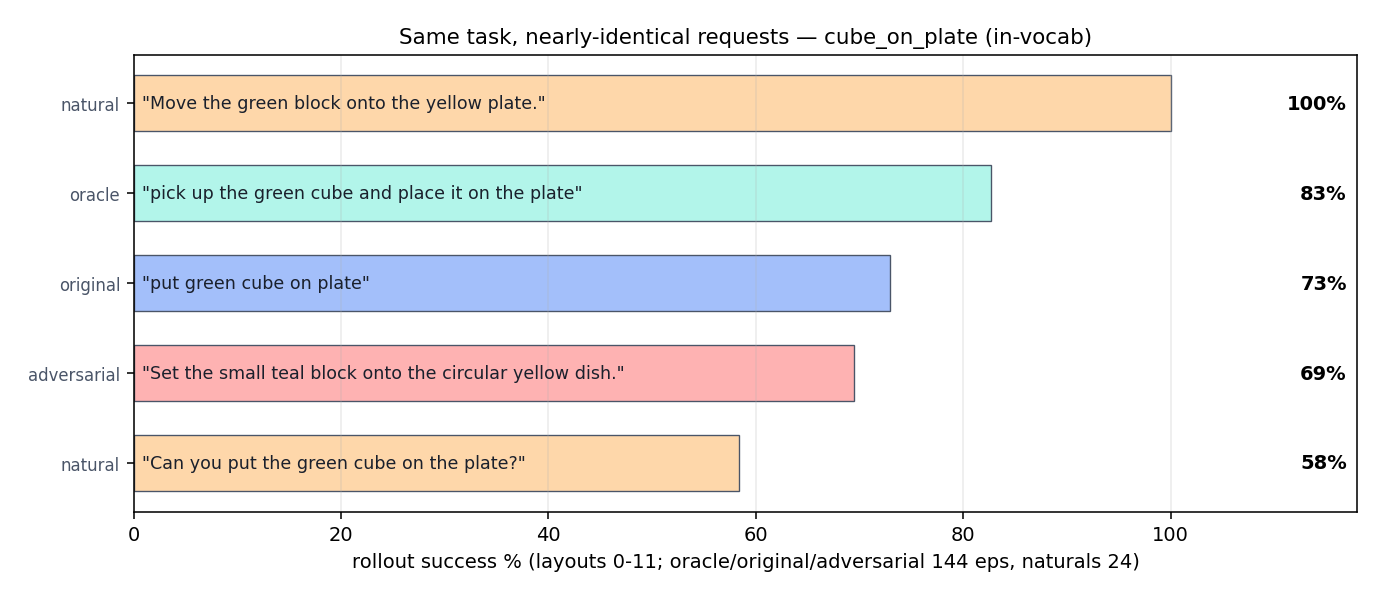
\includegraphics[width=\columnwidth]{spread_cube_on_plate.png}
    \caption{}
    \label{fig:spread_cube_on_plate}
\end{figure}

\begin{figure}[!t]
    \centering
    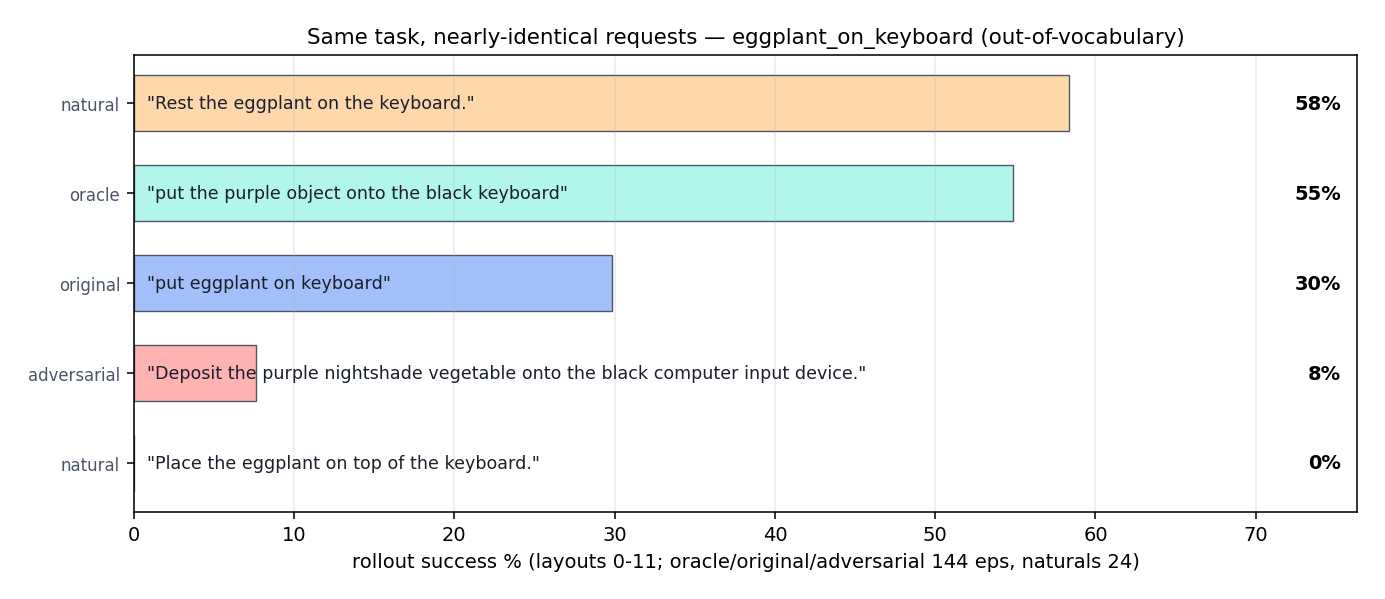
\includegraphics[width=\columnwidth]{spread_eggplant_on_keyboard.png}
    \caption{}
    \label{fig:spread_eggplant_on_keyboard}
\end{figure}

In an attempt to address these issues we add a \textit{translator} model that translates incoming task-instructions into (what is ideally) the robot's preferred form. We try three different methods. Each of our methods inspects the robot's training data and optionally some simulated rollouts of various task rephrasings.

Our first and most successful method we call \textit{LLM-derived rules}. In this method, we first calculate VLA task success across many different task phrasings. We perform this phrase-comparison for both its real-world training set and in a simulated environment. Since we cannot directly measure task success on the robot's real-world training data, we use a gripper-based proxy. This proxy shows high correlation with actual task success, especially when sampled at many different frames along a robot's task trajectory. After gathering a dataset of per-task phrase-rankings, we ask an LLM to derive observations about how phrasing affects task success. These observations are compiled into rules, and the rules are given in a prompt to an off-the-shelf VLM (Vision Language Model) rephraser. This is the method reported in the abstract; it improves VLA performance on adversarially phrased instructions by 25\% and improves performance on naturally phrased instructions by 30\%.

Our second method is more or less the "weights" based, RL counterpart to the above. In this method, we test many rephrasing per task, ranking the results according to our gripper-based proxy reward and apply GRPO. We have yet to see significant improvement when using this method, though it does seem that the proxy reward is able to be mildly optimized.

Our third method trains a VLM to map rephrased training tasks back to their original training task. In our evaluation, it helps with in-vocabulary tasks and hurts on out-of-vocabulary tasks. For future work, it may be interesting to endow this method with access to our proxy-reward function; in about half of all training tasks, our proxy was able to find a better task phrase than the original.







\section{Related Work}

\textbf{Language-Sensitivity. }
Other works call attention to the language-sensitivity of language-conditioned robot policies ~\cite{karnik2024embodied}.

\textbf{Reducing Language Sensitivity. }
Recent works improve VLA performance by augmenting its training data with additional rephrases of its training instructions ~\cite{kwok2026scaling, chen2026steerable}.

In conjunction with the above, a frozen VLA's performance can be improved by generating many phrase-action pairs at runtime and then using a pre-trained model to select the best candidate ~\cite{kwok2026scaling}. This method is our closest known comparison, yet we operate solely on task-phrasing; that is, we do not explicitly select good candidate actions. Moreover, though generating multiple phrase-action pairs at each inference step is relatively inexpensive, we avoid this cost by generating our rephrase just once, at the beginning of the episode.

\textbf{Using a VLM to improve VLA performance. }
Another body of work incorporates a VLM in some capacity to improve the performance of a downstream VLA \cite{zitkovich2023rt2,driess2023palme,shi2025hirobot}.

TODO: write more about methods that take into account capabilities of the robot (eg Saycan)



\section{Method}
\label{sec:method}

Vision-Language-Action models are highly sensitive to the phrasing of
their instructions, even when task semantics are unchanged. We propose
inserting a \emph{rephraser} between the user and the executor
(Fig.~\ref{fig:deployment}) that translates each incoming instruction
into the executor's preferred phrasing, leaving the executor itself
frozen. We first build the instruments for characterizing phrase
sensitivity (\S\ref{sec:characterizing}) and select a reward function
for scoring candidate phrasings (\S\ref{sec:reward}); we then present
three methods of increasing training commitment for learning the
rephraser (Fig.~\ref{fig:training_flow_compact}).

\subsection{Characterizing Phrase Sensitivity}
\label{sec:characterizing}

\textbf{Oracle Phrase Search.}
To upper-bound what phrasing alone can contribute, we search for each
task's best-performing instruction: a pool of candidate rewordings
(LLM-proposed paraphrases and systematic variants of the nominal
instruction) is rolled in simulation, and the candidate with the
highest success rate on a selection split of scene layouts is retained
as that task's \emph{oracle phrasing}. To limit selection bias, oracle
phrases are selected on 18 of the 24 evaluation layouts and reported on
all 24. The gap between oracle and nominal phrasings measures the
headroom available to any rephrasing method.

\textbf{Adversarial Phrase Generation.}
To lower-bound robustness, we generate adversarial rewordings that
preserve the task goal while avoiding the executor's preferred surface
forms: objects are referenced by description or indirection rather than
their canonical names (e.g.\ ``the plastic-handled eating utensil'' for
a spoon), with scene-plausible attributes added. Rewordings are
authored by an image-conditioned LLM (Gemini,
\texttt{gemini-3.5-flash}, temperature 0.8), seeded with four few-shot
examples of the genre from the INT-ACT release~\cite{intact}; the full
prompt is given in Appendix~\ref{app:ert-prompt}. Importantly, the
adversarial generator used for \emph{evaluation} is distinct from the
model that generates hostile variants for \emph{training}
(\S\ref{sec:sft}), so evaluation attacks are held out from everything
the learned methods see.

\textbf{Natural Phrase Generation.}
Between these extremes, we measure robustness to the phrasing variation
real users produce: $K{=}16$ rephrases of each instruction, generated
by an image-conditioned VLM (Gemini Pro, \texttt{gemini-pro-latest})
prompted for natural, everyday phrasing with no knowledge of the
executor, its training data, or any phrasing heuristics
(Appendix~\ref{app:natural-prompt}). Because the generator sees the
scene, natural rephrases include perceptual re-descriptions (``the blue
cloth'' for a towel) --- a qualitatively different stress than
text-only paraphrasing, and the one deployed systems actually face.

\subsection{Selecting a Reward Function}
\label{sec:reward}

Both the phrase search (\S\ref{sec:search-rules}) and RL
(\S\ref{sec:grpo}) require scoring a candidate phrase by how well the
executor performs when conditioned on it, in two regimes
(Fig.~\ref{fig:training_flow_compact}).

\textbf{Simulated success-rate.}
Where a task is simulatable, the score is the empirical success rate of
the frozen executor conditioned on the candidate phrase, rolled over a
fixed set of scene layouts. This is the ground-truth signal, but it is
expensive and unavailable for tasks that exist only as real-world
demonstrations.

\textbf{A gripper-error proxy from ground-truth trajectories.}
For the non-simulatable regime we score a phrase by how well the
phrase-conditioned executor reconstructs recorded expert trajectories:
at $F$ sampled frames of $C$ demonstration episodes, we query the
frozen executor and measure the error of its predicted
\emph{gripper-channel} actions against the ground truth --- whether the
phrase triggers correct grasp/release behavior at the correct moments.
Downstream consumers use rewards only through within-group rankings, so
only the ordering of phrases matters. We also evaluated a learned
verifier over the executor's full action features; it was equal to or
worse than the gripper signal at higher sampling rates, so we use
gripper-only for simplicity (Appendix~\ref{app:reward-grids}).

\textbf{Validation and budget allocation.}
We validated the proxy on four simulatable tasks. For two, real
training demonstrations exist and the training instruction applies
verbatim in simulation (``put the spoon on the towel'', ``put the
green cube on top of the yellow cube''); for the other two, we
generated demonstrations by keeping successful simulated episodes.
In all four, the simulator measures each phrase's true success rate,
while the proxy scores the same phrases by comparing the executor's
predicted actions against the demonstrated actions --- and we count how often the two agree on which of two phrases is
better: 92.4\% on clearly-different pairs, and 79.6\% when true
success differs by only 5--10 points ($F{=}4$, $C{=}20$). More episodes beat more frames
at equal cost, so the search screens cheaply ($F{=}1$, $C{=}4$) and
re-scores finalists carefully ($F{=}4$, $C{=}10$), while RL accepts
noisier scores for throughput ($C{=}5$, $F{=}4$) --- group averaging
washes the noise out.

\begin{figure}[!t]
    \centering
    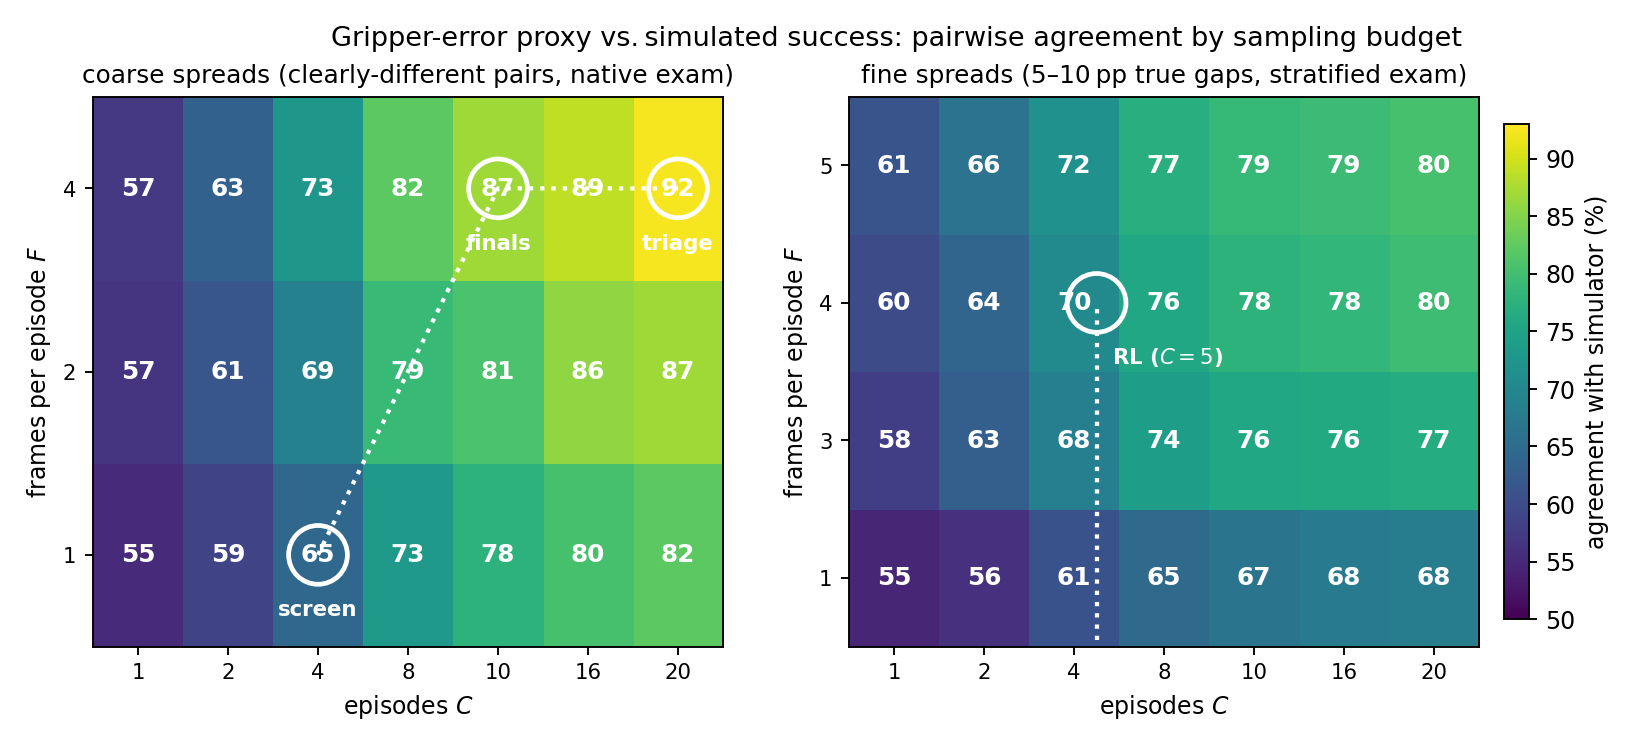
\includegraphics[width=\columnwidth]{reward_grids_gripper.png}
    \caption{Agreement between the gripper-error proxy and simulated
success, by sampling budget ($C$ episodes $\times$ $F$ frames per
episode). Each cell is the fraction of phrase pairs the proxy orders
the same way as the simulator. \emph{Coarse spreads}: pairs whose true
success rates clearly differ (median gap 27\,pp; native-task exam).
\emph{Fine spreads}: pairs differing by only 5--10\,pp. Dotted lines
are level sets of constant total budget $F{\times}C$; along any such
line, tends to be higher with more episodes and fewer frames. The
search screens at ($F{=}1$, $C{=}4$) and re-scores finalists at
($F{=}4$, $C{=}10$); cross-task triage uses up to $C{=}20$; RL runs at
($F{=}4$, $C{=}5$).}
    \label{fig:reward_grids_gripper}
\end{figure}

\subsection{Reward-Guided Phrase Search and LLM Rule Distillation}
TODO: Update this in light of our most recent work.
Make sure to describe the difference between v3 rules and v4 rules, and rename them to something like
"rollout-derived rules" and "rollout + training-data derived rules"

\label{sec:search-rules}
This method runs the loop of Fig.~\ref{fig:training_flow_compact} twice.
The first iteration reuses the oracle search of
\S\ref{sec:characterizing} on simulatable tasks, scoring candidates by
simulated success-rate, and distills the scored phrases into an initial
set of phrasing rules. The second iteration searches the
\emph{training} corpus --- where no simulator is available --- scoring
candidates with the trajectory proxy of \S\ref{sec:reward}, with the
first iteration's rules informing candidate authoring; its results are
distilled, together with the previous rules, into the final rule set.

\textbf{Candidates and task selection.}
Candidate rephrasings are authored by an image-conditioned LLM from the
instruction and a scene frame, guided by the first iteration's rules
and style examples from the oracle search (prompt in
Appendix~\ref{app:search-prompts}); the original is always retained as
a candidate. Search budget goes to the 213 training instructions with
the most recorded episodes, processed in descending order of episode
count --- selecting for score reliability rather than predicted
headroom.

\textbf{Search.}
Within a task, every candidate is scored on the same episodes and
frames and ranked by reward. Eight authored candidates plus the
original are screened cheaply ($F{=}1$, $C{=}4$); the top three are
re-scored with the original at the finals budget ($F{=}4$, $C{=}10$).
The winner then seeds up to two hill-climbing rounds: an LLM proposes
eight variations of the incumbent, all are scored on identical frames,
and a variation is adopted only if it beats the incumbent's
simultaneous re-score by a minimum margin. The output is a per-task
ranking of phrases with their margins over the original.

\textbf{Rule distillation with hypothesis gating.}
An LLM reads the accumulated rankings --- winners, losers, and margins
across tasks --- together with the previous rule set, and proposes
updated rules for how phrasing affects this executor. Proposed rules
are treated as hypotheses: each is tested by applying it to held-out
training instructions and scoring the rewrites with the same reward.
This gate proved decisive. Of 817 elite searched rewrites, only 20.6\%
beat their original, and all 14 candidate \emph{improvement} rules
failed held-out testing (mean $-1.8$\,pp per rule-following rewrite).
The distillation therefore converged on a conservative protocol: the
final rules primarily teach the rephraser to \emph{repair} defective
inputs --- restoring canonical object nouns and training-register
phrasing --- and to leave already-canonical inputs untouched. The full
rule set is reproduced in Appendix~\ref{app:rules}.

\textbf{Deployment.}
The frozen rule set is placed in the prompt of an off-the-shelf VLM,
which rewrites each incoming instruction once, at the start of the
episode (Fig.~\ref{fig:deployment}).

\subsection{Supervised Finetuning (SFT) from Rephrases to Canonical Instructions}
\label{sec:sft}

\subsection{Learning to Rephrase with Group Relative Policy Optimization (GRPO)}
\label{sec:grpo}


\section{Experiments}
\label{sec:experiments}

\subsection{Experimental Setup}
\label{sec:setup}

\textbf{Executors and simulation.}
We evaluate on the SIMPLER suite~\cite{simpler} of WidowX manipulation
tasks in simulation, using the INT-ACT evaluation
stack~\cite{intact}. Our executors are two frozen $\pi_0$
policies~\cite{pi0} fine-tuned on Bridge data~\cite{bridge}: a standard
fine-tune~\cite{kwok2026scaling} and a \emph{rephrase-augmented} fine-tune trained with
paraphrase augmentation~\cite{kwok2026scaling}. Neither executor is updated by any
of our methods; all learning acts on the instruction channel alone.

\textbf{Sealed evaluation suite.}
Our primary benchmark is a \emph{sealed} test suite of 12 tasks
$\times$ 24 scene layouts, frozen before method development and never
used for training, tuning, or prompt iteration. Each evaluation arm
rolls 12 episodes per (task, layout) cell, i.e.\ 3{,}456 episodes per
arm. All arms were preregistered before execution; every phrase set was
inspected before its first exposure to the sealed suite.

\textbf{Vocabulary strata.}
We stratify the 12 sealed tasks by whether their key object nouns occur
in the executor's training corpus: 5 tasks are \emph{in-vocabulary} and
7 are \emph{out-of-vocabulary}. We report pooled success alongside both
strata, since phrasing interventions behave differently when the
canonical noun is unavailable to the executor.

\textbf{Adversarial and natural arms.}
The adversarial arm rolls one adversarial rewording per task
(\S\ref{sec:characterizing}) over the full grid: 12 instructions
$\times$ 24 layouts $\times$ 12 repetitions (3{,}456 episodes). The
natural-rephrase arms roll all $K{=}16$ natural rephrases per task over
12 layouts, one episode each (2{,}304 episodes per arm), reporting on
all 24 layouts where noted.

\textbf{Development and validation sets.}
Method development, reward-function selection, and RL monitoring use
separate training tasks and a fixed validation probe (8 tasks $\times$
24 layouts, one episode each); no sealed task--layout cell is ever used
for development.

\textbf{Metrics.}
We report task success rate (\%) under SIMPLER's per-task success
criteria, pooled over tasks and stratified by vocabulary. At
$n=3{,}456$ episodes per sealed arm, the standard error of a pooled
rate near 35\% is ${\sim}0.8$ percentage points.

\subsection{How Phrase-Sensitive Are VLAs?}     % answers III-A: oracle
\label{sec:results-sensitivity}                 % headroom, adversarial drop,
                                                % natural-rephrase penalty

\subsection{Comparing the Three Learning Methods}  % rules vs SFT vs GRPO
\label{sec:results-comparison}                     % on sealed + robustness,
Probably here we should have a brief intro comparing the three methods.

Then we can have a sub-sub section on each of the methods, showing results and analyzing.

We should rename v3 and v4 rules accordingly. We



\subsection{Analysis}                    % template x applier matrix, rules x
\label{sec:results-analysis}             % executor interaction, RL training
                                         % dynamics (the inverted-U curve)


\section{Conclusions}
Our LLM-based loop seemed better able to generalize than our classic RL or SFT loop.
In light of this, should be reconsider improvements to our traditional weights-based RL
algorithms that somehow generalize better?

Future-work:
- get a weights-based RL algorithm to work more effectively
- more thorough running of the rules iteration loop -- we only did a few ad hoc iterations
and it would be nice to better automate it
- we should test different models and datasets, as well
- these methods are applied to rephrasing, but it could be equally as interesting
to apply them to planning as well



\addtolength{\textheight}{-12cm}   % This command serves to balance the column lengths
                                  % on the last page of the document manually. It shortens
                                  % the textheight of the last page by a suitable amount.
                                  % This command does not take effect until the next page
                                  % so it should come on the page before the last. Make
                                  % sure that you do not shorten the textheight too much.

%%%%%%%%%%%%%%%%%%%%%%%%%%%%%%%%%%%%%%%%%%%%%%%%%%%%%%%%%%%%%%%%%%%%%%%%%%%%%%%%



%%%%%%%%%%%%%%%%%%%%%%%%%%%%%%%%%%%%%%%%%%%%%%%%%%%%%%%%%%%%%%%%%%%%%%%%%%%%%%%%



%%%%%%%%%%%%%%%%%%%%%%%%%%%%%%%%%%%%%%%%%%%%%%%%%%%%%%%%%%%%%%%%%%%%%%%%%%%%%%%%
\section*{Appendix}
\section{Natural-Rephrase Generation Prompt}
\label{app:natural-prompt}

Natural rephrases are generated with Gemini Pro
(\texttt{gemini-pro-latest}, accessed August 2026) at temperature 1.0,
two sampled calls of 8 rephrases per instruction, deduplicated
(case-insensitive) to $K{=}16$. The scene image is attached to each
call. The prompt deliberately contains no information about the
executor, its training data, or any phrasing heuristics; the only
register target is natural human phrasing.

\vspace{4pt}
\noindent\textit{System prompt:}
\begin{quote}\small\ttfamily
You are a text-transformation assistant for robot manipulation tasks.\\[3pt]
You will be given:\\
- An image of the scene.\\
- An instruction describing a manipulation goal.\\[3pt]
Your task is to:\\
1. Understand the meaning of the original instruction.\\
2. Reword the instruction into multiple alternatives that preserve the
original intent.\\[3pt]
Guidelines:\\
- Every reworded instruction must be something a person might actually
say when asking for this task to be done.\\
- All reworded instructions must mean the same thing as the original.
\end{quote}

\noindent\textit{User prompt (per instruction, image attached):}
\begin{quote}\small\ttfamily
Given the original instruction: "\{src\}", and the attached image,
generate 8 reworded instructions that convey the same objective.\\[3pt]
Guidelines for rephrasing:\\
1. Write the way real people actually talk when asking for a task ---
natural, everyday phrasing.\\
2. Different people phrase the same request differently: vary the
phrasing the way different natural speakers would.\\
3. Each rephrase must keep the same objects and the same goal as the
original.\\
4. You may refer to objects the way they appear in the image, but do
not contradict the original instruction or mention things you cannot
see.\\[3pt]
Format your response as (no analysis, no commentary):\\
Reworded Instructions:\\
1. <Alternative phrasing 1>\\
...\\[3pt]
Original Instruction:\\
\{src\}
\end{quote}

\section{Adversarial Instruction Generation Prompt}
\label{app:ert-prompt}

Sealed adversarial instructions are authored by Gemini
(\texttt{gemini-3.5-flash}, temperature 0.8), one per task, with the
scene image attached. \texttt{\{shots\}} is filled with four
\mbox{nominal $\rightarrow$ ERT} example pairs taken verbatim from the
INT-ACT release's extreme-rephrasing examples~\cite{intact};
\texttt{\{nominal\}} is the task's nominal instruction. The first line
of the response is kept.

\begin{quote}\small\ttfamily
You are building an Extreme Rephrasing Test (ERT) for robot
instructions: adversarial rewordings that keep the task goal but are
maximally hostile to a language-conditioned robot policy. The attached
image shows the actual scene. Reference objects by description or
indirect means rather than their plain names, add scene-plausible
attributes, keep the SAME goal. Examples of the genre:\\
\{shots\}\\[3pt]
Nominal instruction: "\{nominal\}"\\
Produce exactly ONE complete ERT rephrasing (output just the
instruction, no quotes, no explanation).
\end{quote}

\section{Phrase-Search Prompts}
\label{app:search-prompts}

\noindent\textit{Candidate generation (one call per instruction, scene
image attached; \{shots\} holds three style examples from the val-set
oracle search):}
\begin{quote}\small\ttfamily
You are helping phrase instructions for a robot arm policy trained on
kitchen-manipulation demonstrations (BridgeData). The attached image
shows the robot's actual camera view for this task.\\
Current instruction: "\{nominal\}"\\
Write 8 alternative phrasings the policy is likely to follow RELIABLY.
Guidelines learned from prior experiments:\\
- Name objects with common household words the training data would
contain; if an object's name is unusual, rename it to what it looks
like (e.g. "ramekin" -> "white bowl").\\
- Add concrete color/appearance adjectives ONLY for objects visible in
the image.\\
- Keep the imperative form and the same task meaning. Keep each under
15 words.\\
- Vary structure across the 8 (some minimal edits, some full
rewrites).\\
Style examples of phrasings that performed well elsewhere:\\
\{shots\}\\
Output exactly 8 lines, one phrasing per line, no numbering, no quotes.
\end{quote}

\noindent\textit{Hill-climb variation (per round, image attached):}
\begin{quote}\small\ttfamily
The attached image is a robot arm's camera view. The current
best-performing instruction phrasing for this scene is:\\[2pt]
"\{seed\}"\\[2pt]
Write \{k\} close VARIATIONS of this phrasing that might work even
better for a robot policy trained on kitchen-manipulation
demonstrations: keep its winning structure but vary object adjectives,
object names (common household words, matching what is visible), and
verb choice. Keep each under 15 words, imperative form, same task
meaning.\\
Output exactly \{k\} lines, one per line, no numbering, no quotes.
\end{quote}

\section*{ACKNOWLEDGMENT}



%%%%%%%%%%%%%%%%%%%%%%%%%%%%%%%%%%%%%%%%%%%%%%%%%%%%%%%%%%%%%%%%%%%%%%%%%%%%%%%%


\begin{thebibliography}{99}

\bibitem{kwok2026scaling}
J. Kwok, X. Zhang, M. Xu, Y. Liu, A. Mirhoseini, C. Finn, and M. Pavone,
``Scaling verification can be more effective than scaling policy learning for vision-language-action alignment,''
\emph{arXiv preprint arXiv:2602.12281}, 2026.

\bibitem{chen2026steerable}
W. Chen, J. S. Bhatia, C. Glossop, N. Mathihalli,
R. Doshi, A. Tang, D. Driess, K. Pertsch, and S. Levine,
``Steerable vision-language-action policies for embodied
reasoning and hierarchical control,''
\emph{arXiv preprint arXiv:2602.13193}, 2026.

\bibitem{karnik2024embodied}
S. Karnik, Z.-W. Hong, N. Abhangi, Y.-C. Lin,
T.-H. Wang, and P. Agrawal,
``Embodied red teaming for auditing robotic foundation models,''
\emph{arXiv preprint arXiv:2411.18676}, 2024.

\bibitem{ahn2022saycan}
M. Ahn, A. Brohan, N. Brown, Y. Chebotar, O. Cortes,
B. David, C. Finn, C. Fu, K. Gopalakrishnan, K. Hausman,
\emph{et al.},
``Do as I can, not as I say: Grounding language in robotic
affordances,''
in \emph{Proc. 6th Conf. Robot Learning (CoRL)}, 2022.

\bibitem{zitkovich2023rt2}
B. Zitkovich, T. Yu, S. Xu, P. Xu, T. Xiao, F. Xia,
J. Wu, P. Wohlhart, S. Welker, A. Wahid, \emph{et al.},
``RT-2: Vision-language-action models transfer web knowledge
to robotic control,''
in \emph{Proc. Conf. Robot Learning},
pp. 2165--2183, 2023.

\bibitem{driess2023palme}
D. Driess, F. Xia, M. S. M. Sajjadi, C. Lynch,
A. Chowdhery, B. Ichter, A. Wahid, J. Tompson,
Q. Vuong, T. Yu, W. Huang, Y. Chebotar, P. Sermanet,
D. Duckworth, S. Levine, V. Vanhoucke, K. Hausman,
M. Toussaint, K. Greff, A. Zeng, I. Mordatch,
and P. Florence,
``PaLM-E: An embodied multimodal language model,''
in \emph{Proc. 40th Int. Conf. Machine Learning (ICML)},
2023.

\bibitem{shi2025hirobot}
L. X. Shi, B. Ichter, M. Equi, L. Ke, K. Pertsch,
Q. Vuong, J. Tanner, A. Walling, H. Wang, N. Fusai,
\emph{et al.},
``Hi Robot: Open-ended instruction following with hierarchical
vision-language-action models,''
in \emph{Proc. 42nd Int. Conf. Machine Learning (ICML)},
2025.

\bibitem{simpler}
X. Li, K. Hsu, J. Gu, K. Pertsch, O. Mees, H. R. Walke, C. Fu,
I. Lunawat, I. Sieh, S. Kirmani, S. Levine, J. Wu, C. Finn, H. Su,
Q. Vuong, and T. Xiao,
``Evaluating real-world robot manipulation policies in simulation,''
in \emph{Proc. Conf. Robot Learning (CoRL)}, 2024.

\bibitem{intact}
I. Fang, J. Zhang, S. Tong, and C. Feng,
``From intention to execution: Probing the generalization boundaries of
vision-language-action models,''
\emph{arXiv preprint arXiv:2506.09930}, 2025.

\bibitem{pi0}
K. Black, N. Brown, D. Driess, A. Esmail, M. Equi, C. Finn, N. Fusai,
L. Groom, K. Hausman, B. Ichter, S. Jakubczak, T. Jones, L. Ke,
S. Levine, A. Li-Bell, M. Mothukuri, S. Nair, K. Pertsch, L. X. Shi,
J. Tanner, Q. Vuong, A. Walling, H. Wang, and U. Zhilinsky,
``$\pi_0$: A vision-language-action flow model for general robot control,''
\emph{arXiv preprint arXiv:2410.24164}, 2024.

\bibitem{bridge}
H. Walke, K. Black, A. Lee, M. J. Kim, M. Du, C. Zheng, T. Zhao,
P. Hansen-Estruch, Q. Vuong, A. He, V. Myers, K. Fang, C. Finn, and
S. Levine,
``BridgeData V2: A dataset for robot learning at scale,''
in \emph{Proc. Conf. Robot Learning (CoRL)}, 2023.

\bibitem{qwen}
Qwen Team,
``Qwen3 technical report,''
\emph{arXiv preprint arXiv:2505.09388}, 2025.





\end{thebibliography}




\end{document}
